\section{Unavoidable Hazards of Bureaucracy\label{sec:unavoidable-hazards}}


% TODO: For each of the unavoidable hazards, how is this a natural consequence of the definition of bureaucracy
% TODO: What is the best response to handle this problem

There are certain challenges in a bureaucracy that cannot be avoided. The value of recognizing them is to understand that what you're experiencing isn't an anomaly. The problem isn't unique to you, your circumstances, your coworkers, or the organization. The cause is the combination of all those factors.
Understanding the unavoidable hazards in a bureaucratic organization improves your Process Empathy. 

Accounting for unavoidable hazards is what distinguishes being na\"ive from having experience. A na\"ive bureaucrat may see a challenge and come up with an idea of how to improve the situation. In practice, merely having a good idea is insufficient for improvement; the availability of a good idea is not enough for adoption or continuation if there are incentives for stakeholders contrary to the idea. 

Even when a good idea is adopted that does not imply longevity. The idea may only be enacted for a promotion, or while the champion persists. Concepts that improve a team or organization do not need to continue. 

Being aware of the unavoidable hazards is vital to your tenacity as a bureaucrat. Your emotional fortitude is critical. 


\ \\
\begin{samepage}
\textit{Hazard}: \textbf{Separation of responsibility and accountability}. \\
Each bureaucrat in an organization has responsibilities associated with their role. The ability to complete the tasks associated with the role is not wholly within the scope of the bureaucrat's control. You are dependent on other bureaucrats. Even if there is a desire for action, the action might not be immediately feasible because of a dependence on another person or process. 

The consequence of separating responsibility from authority is that other people look incompetent or lazy and unresponsive. For the same reasons, you feel impotent. In this scenario Process Empathy can take two forms: empathizing with fellow bureaucrats who are in this state, or intentionally exceeding the boundaries of your role to break the equilibrium. 
\end{samepage}

\ \\
\begin{samepage}
\index{mantra!perception matters more than intent}
\textit{Hazard}: \textbf{Perception matters more than intent}. \\
You may mean to convey a specific message, but the way your listeners hear that content or read the message depends on context and interpretation. 
Decreasing the ambiguity in phrasing is a useful investment, but you don't control how an audience responds. 

Communication is crucial for bureaucracy, so the best response is iterating with an audience rather than expecting a single message to be enough. 
\end{samepage}

\ \\
\begin{samepage}
\textit{Hazard}: \textbf{Appreciation for being an effective bureaucrat is rare.}\\
If you do your job well no one will notice. This is because of an expectation of smooth and fast interactions. Frictionless engagement is expected even if that is not the norm. 

Consider teachers who catch cheating students~\cite{2022_unknown}:
\begin{quote}
``No one [thanks teachers] for policing cheating. Not the cheaters, not the honest students who feel inconvenienced and mistrusted, and certainly not the school [administrators] who have to process academic dishonesty paperwork.''
\end{quote}
\end{samepage}

This same concept applies to any bureaucrat. The number of thank you cards sent to \href{https://www.fda.gov/}{Food and Drug Administration} meat inspectors keeping food safe, \href{https://www.osha.gov/}{Occupational Safety and Health Administration} regulators ensuring a safe work environment, \href{https://www.fcc.gov/}{Federal Communications Commission} detecting disruptive electromagnetic signals, \href{https://www.ftc.gov/}{Federal Trade Commission}, and \href{https://www.sec.gov/}{Securities and Exchange Commission} is likely small.\footnote{FoIA 2022-000758 submitted to the \href{https://www.fcc.gov/}{Federal Communications Commission}  
sought the first 100 documents received by the FCC from consumers with any of the words ``thank,'' ``thanks,'' ``appreciate,'' or ``appreciated'' between January 1, 2020 to December 31, 2020. 
I reviewed the 100 documents and found no letter of gratitude; just complaints.}
% POTENTIAL task: ask each agency how many thank you letters they receive
% FOIA SSA-2022-01  5009
% FOIA FCC-2022-000758

There are counterexamples in public service bureaucracy. 
Law enforcement is thanked when there is a victim of a crime. 
\index{exemplar!law enforcement officers}
The military is held in high regard. 
\index{exemplar!military}
In both of those bureaucracies the bureaucrats are visible and the consequence of their work is tangible. 

In large organizations there are teams of bureaucrats like the Information technology department and human resources. IT support bureaucrats are occasionally thanked by their subjects, though most of the time the expectation is that computers should just work. Outside of hiring, HR produces few tangible products, so the appreciation is lower.


\ \\
\begin{samepage}
\textit{Hazard}: \textbf{Lack of accountability to fellow bureaucrats who rely on you.}\\
You are more likely to feel accountable to your supervisor. Performing for your supervisor and explaining your value matters more than the work done to support coworkers.  This also applies when you depend on other people -- they aren't accountable to you.

To counter this tendency, build personal relationships with peers. This requires ongoing investment, both to maintain relationships and to create bonds with new coworkers as your previous coworkers leave.
\end{samepage}

\ \\
\textit{Hazard}: \textbf{Decision-makers are under-informed and inexperienced.}\\
You can make a decision with insufficient information. There is rarely an expectation of expertise or experience. 
Gathering information takes time and is thus burdensome.
Having experience requires getting experience -- you either start as a novice and make mistakes, have formal academic training, or rely on mentorship to avoid the direct experience of mistakes.

\ \\
\begin{samepage}
\textit{Hazard}: \textbf{Gathering data for decisions takes resources and expertise.}\\
When there is a desire to gather data, and there is data available to be gathered, an investment of time is necessary. Well-informed decisions take time, experience, or both.
\end{samepage}

\ \\
\textit{Hazard}: \textbf{Defining success is subjective and dynamic}. \\
Who defines success and for which audience in a bureaucratic organization is subjective because of the lack of feedback mechanisms. Consequences may not be immediately obvious. Worse, how success is defined can be changed at any time -- there's no need for consistency. 

\ \\
\begin{samepage}
\textit{Hazard}: \textbf{Change threatens incumbents}. \\
For example, change of plans, roles, tasks, resources, the flatness of the organization, scope, or technology. 
\end{samepage}

Practicing Process Empathy means having compassion towards the fear other people fear and socializing the change before enacting change. This investment in a preview is called \href{https://en.wikipedia.org/wiki/Nemawashi}{nemawashi}.
\index{Wikipedia!nemawashi@\href{https://en.wikipedia.org/wiki/Nemawashi}{nemawashi}}
\iftoggle{WPinmargin}{\marginpar{$>$Wikipedia: Nemawashi}}{}


\ \\
\begin{samepage}
\textit{Hazard}: \textbf{\href{https://en.wikipedia.org/wiki/Diffusion_of_responsibility}{Diffusion of responsibility} 
\index{Wikipedia!diffusion of responsibility@\string\href{https://en.wikipedia.org/wiki/Diffusion_of_responsibility}{diffusion of responsibility}}
in the bureaucracy}. \\
A specific task needs to be completed, and action requires the involvement of multiple collaborators. In this scenario there's a risk of each \gls{participant} not feeling ownership over the outcome. This risk is more likely when roles are less well-defined or when participants don't have relationships to maintain. 
\end{samepage}

Consider the perspectives of an office worker, an office manager, a building manager, an electrical substation operator, and an electrical grid operator.
\begin{center}
\begin{figure}
    \centering
    % left> <lower> <right> <upper
    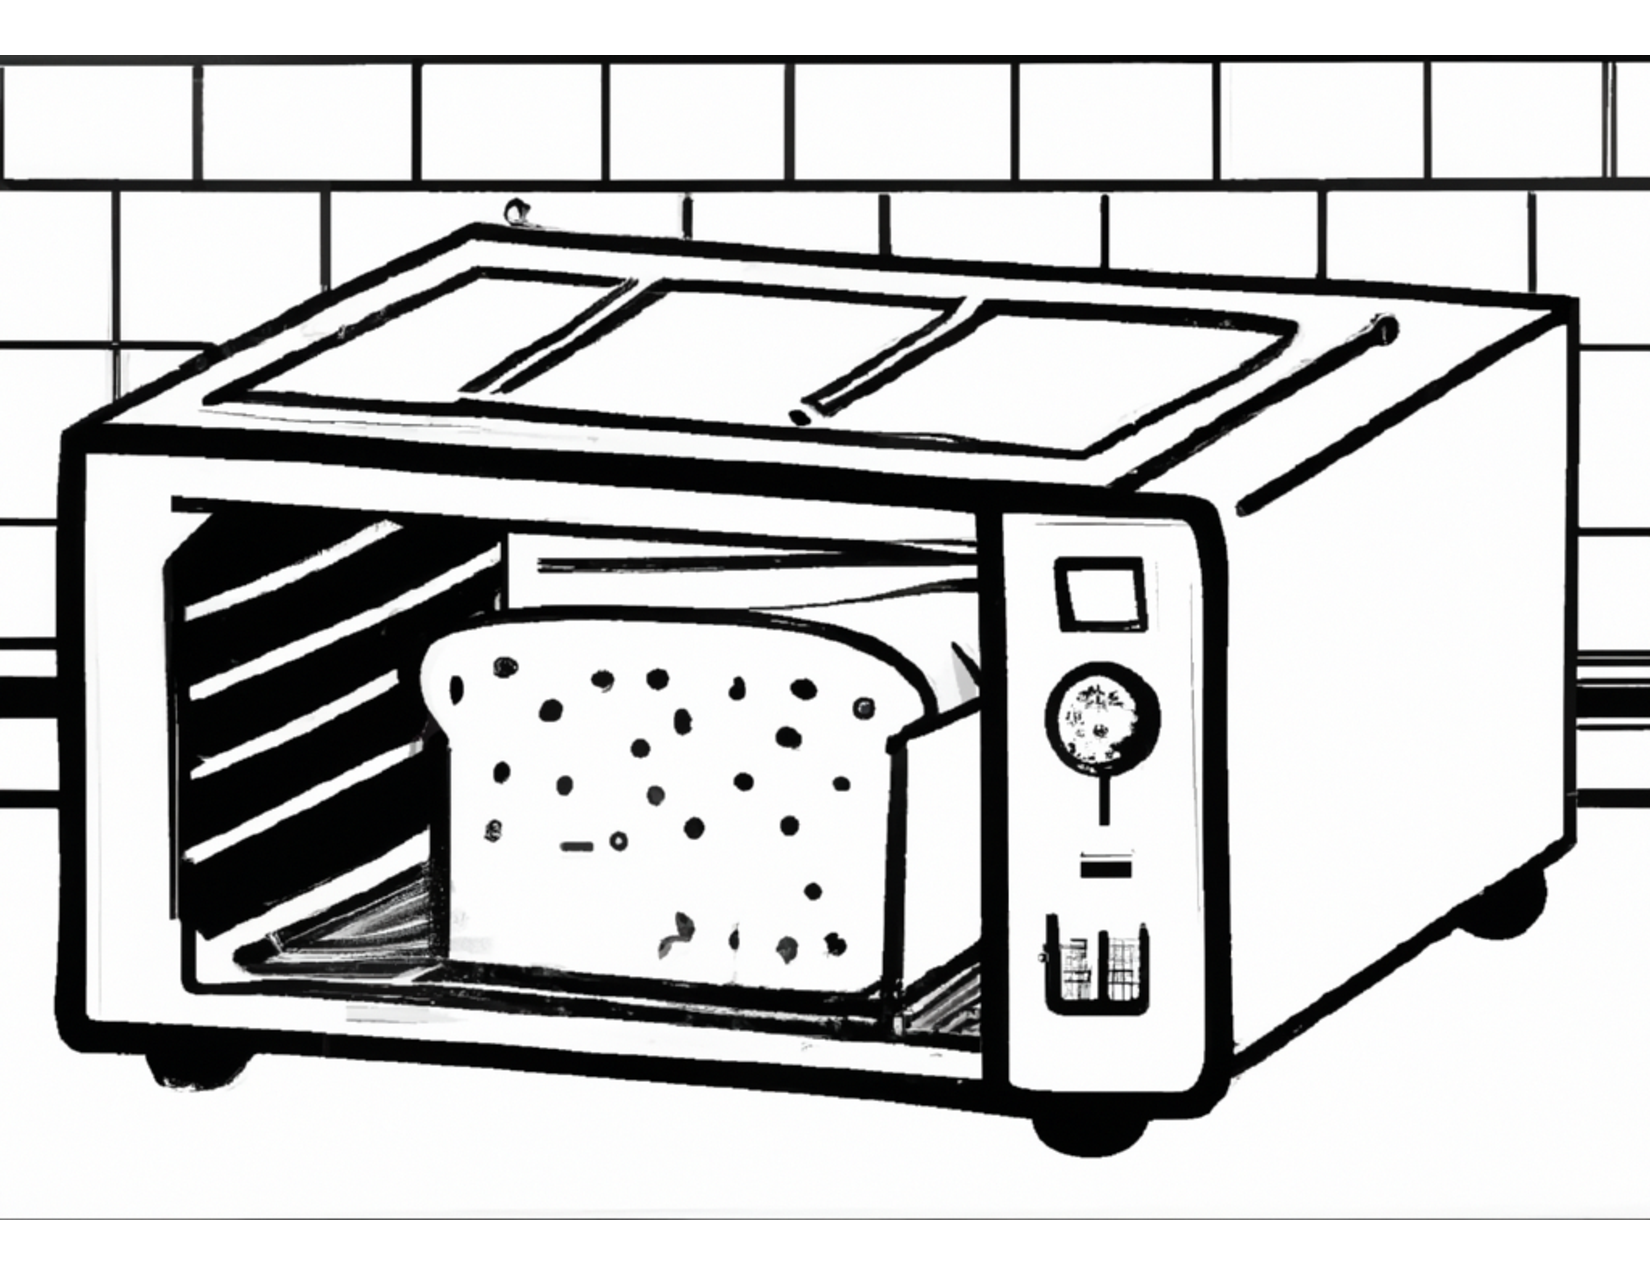
\includegraphics[width=0.7\textwidth,trim={0 2cm 0 0},clip]{images/toaster_oven_in_office_kitchen.pdf}
    \caption{Toaster oven in the office kitchen. Each participant in the accounting process adds overhead to the baseline.}
    \label{fig:toaster_oven}
\end{figure}
\end{center}

%\marginpar{[Tag] Story Time}
\index{story time!layers of margins}
%\begin{storytime}{Layers of Margins}
\begin{mdframed}[frametitle={Layers of Margins},frametitlerule=true,frametitlealignment=\centering]
An office worker wants to plug in a toaster oven in the office kitchen (see Figure~\ref{fig:toaster_oven}). The owner of the toaster oven files a notice with the office manager who tracks electrical loads in the kitchen. 
The toaster owner uses the power number (1200 \href{https://en.wikipedia.org/wiki/Watt}{Watts}) 
\index{Wikipedia!Watt@\href{https://en.wikipedia.org/wiki/Watt}{Watts}}%
from the manufacturer's website. In practice, the toaster oven doesn't  use that much power; that's just the maximum rating for the device. 

The office manager aggregates power from the devices in the kitchen. The office manager has a power budget for the team's kitchen equipment and keeps a margin of 10\% spare capacity for flexibility. The office manager's power budget is provided to the building manager (who keeps a margin of 10\% for flexibility). The building is one of many sharing the electrical substation. The electrical substation owner sees the power consumption is below the rated capacity, but the subscription for available power is full -- no new users can be supported.
%\end{storytime}
\end{mdframed}
Lesson: in a system of aggregated layers, each person only sees adjacent layers. When each person builds safety into their budget, the accumulated slack is excessive and wasteful.

Similar situations arise for temporal planning (schedule), financial budgets, and spatial planning. 

%Once responsibility is assigned, the new risk is that of blame.

\ \\
\textit{Hazard}: \textbf{Diffusion of blame in the bureaucracy}. \\
Example: if something goes wrong, who is at fault: the creator of a policy or the person tasked with executing the policy?

To apply your Process Empathy redirect the focus from blaming people to identifying systemic causes. Did the people involved have enough training? Was adequate time allocated for the task? Were people distracted, tired, or hungry? 

\ \\
\textit{Hazard}: \textbf{Management doesn't do their job well}. \\
From your perspective as a bureaucrat (or subject), management may seem inadequate. The Peter Principle~\cite{1970_Peter}, the Dilbert Principle~\cite{1997_Adams}, and the Gervais Principle~\cite{2009_Rao} all attempt to explain this feature. Process Empathy provides another perspective. 


Management may oversee multiple different disciplines (e.g., engineering, marketing, manufacturing) and different types of people (e.g., outgoing, introverted, independent) and as a result have insufficient time to address everyone's needs.

Management is supposed to facilitate coordination in the hierarchy between teams. Management often lacks technical expertise and lacks time needed to understand each issue deeply. Management adds latency to the process of coordination. The alternative, not including management in coordination and instead relying on direct interaction between peers, is chaotic.

Manage is supposed to coordinate up, down, and laterally. Each of those is supposed to be bidirectional.

Management is supposed to make decisions that affect multiple different teams but lacks expertise and the time to understand each issue in-depth.

Management has a holistic perspective to identify gaps and inefficiencies. Management has the authority to redirect resources to address these issues.

The choice of the manager is to either dive deeply into one topic (and neglect the other needs) or try and superficially respond to all needs and seem like a dilettante. Because management cannot address issues satisfactorily, they appear incompetent.


%The action associated with the observation that management isn't leadership is that there is a void to fill and the void is addressed by influence without authority

%One option is to separate the narrow subject matter experts from the roles of management listed above. Another option is referred to in academia as citizenship duties. Serving on committees, interviewing applicants, promotion boards, mentoring students. Those are in addition to the duties of teaching and research.


\ \\
\textit{Hazard}: \textbf{Policies are dumb}.\\
There are a variety of reasons for this, but a sampling of the causes includes incompetence, diffused control, and what is valued. 

Incompetence as a source of dumb policies arises for multiple reasons, but a subtle cause for individuals making bad decisions is that information isn't available.

As another cause for dumb policies, sometimes the information exists and relevant decisions are identified but control is spread across the organization resulting in lack of coordination. This is a coordination issue.

In some organizations adding complexity is perceived as a source of value. 
This is because nuance (appropriate to a situation) gets confounded with complexity. 

Dumb policies arise when the conventional process is story-driven requirements (as opposed to experimental data).


\ \\
\textit{Hazard}: \textbf{High latency feedback}. \\
See 
\hyperref[sec:slowing-communication]{slow communication}\iftoggle{haspagenumbers}{ on page~\pageref{sec:slowing-communication}}{ } 
and 
\hyperref[sec:decision-delay]{decision delay}\iftoggle{haspagenumbers}{ on page~\pageref{sec:decision-delay}.}{.}

\ \\
\textit{Hazard}: \textbf{Weak feedback}. \\
Suppose my bureaucratic task depends on a service provided by you, a fellow bureaucrat. If your computer isn't working, your ability to provide the service is blocked by a dependency on a computer repair person. You might feel relieved -- you can relax while you wait on the computer repair and you don't have to do work providing the service to me. You might feel anxious -- you're unable to provide the service until the computer is fixed. Regardless of how you feel about the situation, my task is blocked. If neither you nor I have priority relative to the computer repair person's other tasks, then we wait. This question of priority could be resolved hierarchically (for which there is limited attention bandwidth) or socially (dependent on someone having a relationship with the repair person). 

The delay for my task may be sufficiently small that raising the issue through the hierarchy or socially is not a good use of time.

\ \\
\textit{Hazard}: \textbf{The person making the rules that you follow doesn't  know what they're doing}. \\
Your choices then include
\begin{itemize}
    \item Follow the rules that are not correct. This harms your productivity and morale. 
\item You can violate the rules and be more effective. This puts you at risk for sanctions. 
\item You can work the change the rules. Then you are not doing the work that's needed.
\end{itemize}


\ \\
\textit{Hazard}: \textbf{You rarely get to pick who is on the team}. \\
When a task requires collaboration, there is rarely a choice of who you get to work with. 

\ \\
\textit{Hazard}: \textbf{You rarely get to alter team membership.}\\
As a team member, you typically get little input on who you work with. Even as a manager your options for hiring are often limited. 

\ \\
\textit{Hazard}: \textbf{Fear of the unknown.}\\
Current suffering is tolerable compared to the uncertainty of change, especially when the suffering isn't felt by the decision-maker.

By identifying this fear in yourself or those you collaborate with, you can discuss specific concerns and work to address them.
\marginpar{Actionable Advice} 
\index{actionable advice}

\ \\
\begin{samepage}
\textit{Hazard}: \textbf{Fear of change.} \\
Change disrupts the status quo, putting accumulated power at risk and altering relationships. 
\end{samepage}

An emotional basis for decision-making (or avoidance of decision-making) may or may not be rational. Discussing the fear with fellow bureaucrats can ease the burden. 

\ \\
\textit{Hazard}: \textbf{Fear of conflict.}\\
Refers to conflict of ideas, not physical conflict. Conflict of ideas is not personal, though the consequences may have impacts on careers for stakeholders. \\
Professional disagreement is to be expected in a bureaucratic organization.

Feeling uncomfortable is distinct from feeling unsafe. Communicating while feeling discomfort is a useful skill, rather than avoidance. You can show courage by talking about your sense of discomfort. 

\ \\
\textit{Hazard}: \textbf{Inadequate resources: staffing, time, money.}\\
The resources you have to address a challenge may not match the complexity of the issue.

\ \\
\textit{Hazard}: \textbf{Outcomes for the team are ill-defined and constantly shifting.}\\
Most bureaucrats rely on approaches that assume consistency of their environment. Planning for uncertainty and change is more complicated.

\ \\
\textit{Hazard}: \textbf{The reward for good work is more work.}\\
When a coworker doesn't do their fair share, then the productive employee shoulders more burden. The deficient worker has no incentive to improve.

\ \\
\textit{Hazard}: \textbf{The organization has a lack of vision; or has vision but no plan; or has vision and a plan but no consensus; or has vision and a plan and consensus but inadequate resources.}\\
An organization of bureaucrats can operate without a vision, plan, or sufficient resources. Being busy is easy; being productive is hard.
\index{mantra!busy is easy, productive is difficult}

\ \\
\textit{Hazard}: \textbf{Progress depends on subjective decision-making.}\\
Rarely is the optimal path deterministic. 

\ \\
\textit{Hazard}: \textbf{Easier to ask for big money than small money.}\\
Processes are scale invariant. Regardless of whether you're asking for \$1000 or \$100,000, the process is the same. Accountability processes for large amounts of money are not scaled down to fit small amounts because people can be as dumb with \$100 as they are with \$10,000.


\ \\
\textit{Hazard}: \textbf{Some challenges are scale invariant}.\\
Challenges arising from personalities are invariant to where in the hierarchy the problem occurs. The difference is that less attention is paid to the same problem at the lowest levels as compared to higher in the hierarchy because of the scope of impact.
%It doesn't matter how many people you have to manage
%It doesn't matter how many zeros are in your budget


\ \\
\textit{Hazard}: \textbf{Flux of people and processes.} \\
Sources of flux include staff turnover, changing conditions, changing timelines, change of vision, and the need to be promoted. Consistency doesn't yield promotion in a bureaucracy.

\ \\
\textit{Hazard}: \textbf{Why are there so many rules?}\\
To address edge cases and malicious or dumb people. See the \hyperref[table:dilemma-subject-forms]{Dilemma of Forms}.
\marginpar{Page~\pageref{table:dilemma-subject-forms}.}

\ \\
\textit{Hazard}: \textbf{So much paperwork or forms.}
Why is red tape endemic to bureaucracy?\\
Paperwork as a form of coordination in processes to facilitate decentralized decision-making. 

One of the motives for paperwork is to catch people who are misrepresenting their intent, whether accidental or intentional. Documentation makes prosecution more straightforward.

\ \\
\textit{Hazard}: \textbf{Everything is slower.}\\
What the person saying this means is ``slower than desired for what I need" or ``slower than I imagined in my simplified model."

Progress is slower than expected because there aren't as many hours available as na\"ively imagined. The  time spent working in a bureaucracy is less than the number of hours you get paid for. Breaks taken during work, vacation from work, holidays, and sick leave are illustrated in Figure~\ref{fig:hours_per_year}. An added factor is that the people you depend on do not work exclusively on your request -- there are competing investments of attention. 

Developing \gls{process empathy} means having a more detailed model that accounts for the cost of coordination and accounts for there being less time available than the na\"ive expectation. 

% https://rescuetime.wpengine.com/work-life-balance-study-2019/

\begin{figure}[!htb] %[H]
    \centering
    \includegraphics[width=0.9\textwidth]{images/hours_per_activity_per_employed_year}
    \caption{Hours of ``work'' per year when accounting for the rest of life. Assumes five weeks of vacation, two days of sick leave, and eleven holidays.}
    %\href{https://docs.google.com/spreadsheets/d/1ZaOZZXWkEzX4fFltUdlR4A6ENrAXnkzTW4YrjA4tDO8/edit?usp=sharing}{source for calculations}
    % footnotes in caption is not recommended; see https://texfaq.org/FAQ-ftncapt
    % however it can be done; see https://stackoverflow.com/questions/67621322/footnote-in-caption-of-figure-on-latex
    \label{fig:hours_per_year}
\end{figure}

\ \\
\begin{samepage}
\textit{Hazard}: \textbf{Bureaucracy inhibits creativity.}\\
See notes on 
\hyperref[sec:innovation]{innovation}\iftoggle{haspagenumbers}{ on page~\pageref{sec:innovation}.}{ in section~\ref{sec:innovation}.}
\end{samepage}

\ \\
% https://graphthinking.blogspot.com/2017/06/measuring-growth-of-bureaucracy.html
\textit{Hazard}: \textbf{Bureaucracy grows.}\\
Increasing the size of a bureaucracy is easier than cutting it down. 
The causes of growth include
scope creep, an increased number of people participating in the process, an increased workload, or a decrease of the ratio of workers to managers. 

Bureaucracy grows because some people lie -- there are defectors. 
Progress is called ``improved accountability" because we aren't sure who the next liar is going to be.
More work is created for everyone because confronting liars and cheaters is uncomfortable and takes work. 

You can measure the growth of bureaucracy using metrics like the latency in addressing a request and the number of people involved in addressing a request.  

\textbf{Increasing the size of a bureaucracy is easier than cutting it down.}\\


\ \\
% https://graphthinking.blogspot.com/2017/04/growth-of-bureaucracy.html
\textit{Hazard}: \textbf{The ratio of workers to managers gets worse as the size of the hierarchy grows}. \\
As complexity and workload increase, the number of staff needed increases. To facilitate coordination, managers arise. The amount of work being done in a bureaucracy can be small compared to the number of participants.

In Figure~\ref{fig:growth_of_bureaucracy}a, the ratio of workers to participants is 3:3=1. When a manager is added, the ratio is 3:4 = 0.75 (a lower value means less work per employee is being done). Adding a second team with dedicated management puts the ratio at 6:9=0.66. Finally, with a dedicated administrative team (e.g., payroll, hiring, facilities), the ratio is 6:13=0.46.

Adding more people to a hierarchical organization results in diminishing returns for time spent on the central work since bureaucrats invest time maintaining the hierarchy and administrative processes.


% TODO: make a better diagram, 
    \begin{figure}
        \centering
        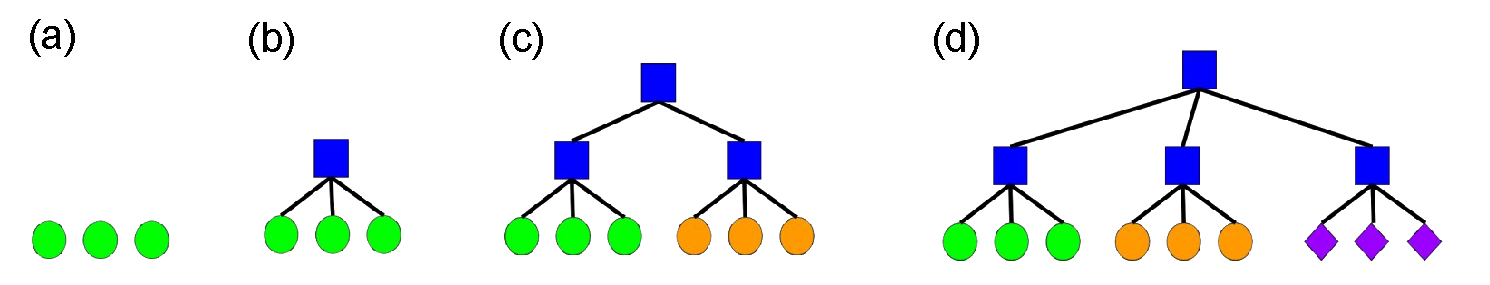
\includegraphics[width=1\textwidth]{images/growth-of-bureaucracy.pdf}
        \caption{Growth of an organization as complexity and workload increase. a: three technical workers 
        \iftoggle{narrowpage}{(dots);}{(green dots);}
         b: administrative functions are delegated to an administrative assistant or manager 
        \iftoggle{narrowpage}{(square);}{(blue square);}
          c: as complexity and scale grow a new technical team 
        \iftoggle{narrowpage}{(dots)}{(orange dots)}
          is brought in with their manager; d: administrative work is delegated to a dedicated team of non-technical staff 
        \iftoggle{narrowpage}{(diamonds).}{(purple diamonds).}
          }
        \label{fig:growth_of_bureaucracy}
    \end{figure}

    \begin{figure}
        \centering
        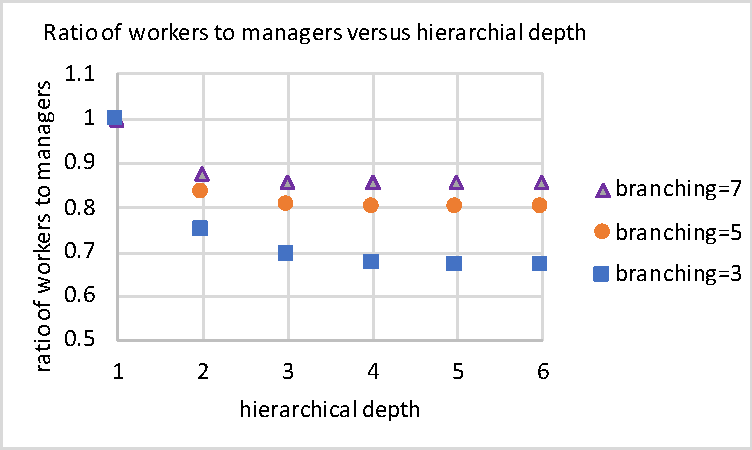
\includegraphics[width=0.8\textwidth]{images/growth-of-bureaucracy-plot.pdf}
        \caption{As the depth of a hierarchical organization increases, the ratio of workers to managers approaches an asymptotic value that depends on the number of workers per manager. The ``branching'' parameter is the number of workers per manager.}
        \label{fig:growth_of_bureaucracy-plot}
    \end{figure}


\ \\
\textit{Hazard}: \textbf{Each person in a bureaucracy has multiple roles}.\\
To limit the expansion of the bureaucracy. The multiple roles come from multiple relationships necessary to span an organization larger than \href{https://en.wikipedia.org/wiki/Dunbar\%27s_number}{Dunbar's number} -- about 150 people. \iftoggle{WPinmargin}{\marginpar{$>$Wikipedia: Dunbar's number}}{ }
\index{Wikipedia!Dunbar's number@\href{https://en.wikipedia.org/wiki/Dunbar\%27s_number}{Dunbar's number}}

\ \\
\begin{samepage}
\textit{Hazard}: \textbf{Everything is more complicated}. \\
Bureaucracy administers access to resources, whether tangible items (water, air) or expertise. There's friction for tangible resources because the easiest solution is you get the resource (without an intermediary). There's friction for expertise because the expert understands things you do not. 
\end{samepage}

\ \\
\textit{Hazard}: \textbf{Bureaucracy is inefficient and wasteful.}\\
The inefficiency of an organization is not just due to a breakdown of communication among its many members. Other sources include 
\begin{itemize}
    \item Individuals in different roles face distinct external incentives that drive a diversity of investments. Work that is not aligned results in wasted effort.
    \item Participants have different views of what constitutes a problem and which problem is most relevant. Coordinating to resolve disagreements appears inefficient regardless of which metric is used to measure efficiency.
    \item Within the organization there can be competition  for resources. Competition leads to wasted effort.
    \item Because decisions by bureaucrats are subjective, there is significant risk of being wrong or being called out by others as being wrong. The incentive to 
\href{https://en.wikipedia.org/wiki/Cover_your_ass}{cover your ass}\footnote{``The 
preferred options are to make sure somebody else does the failing, or to elegantly explain why it looks like a failure, sounds like a failure, but is actually a brilliant advance in an unexpected direction.''~\cite{1996_unknown}}
\index{Wikipedia!cover your ass@\href{https://en.wikipedia.org/wiki/Cover_your_ass}{cover your ass}}\iftoggle{WPinmargin}{\marginpar{$>$Wikipedia: Cover\\your ass}}{}
exists for decisions. As a result, unnecessary work is carried out to limit blame. 
\item Situations and constraints change faster than the time it takes to complete a task.  Then you are faced with either continuing under the initial assumptions or pivoting a project partway through. If an objective quantitative measure of value is available, the return on investment could be determined.
\end{itemize}


Efficiency is typically assessed from the perspective of a serial process -- a single worker could do this task faster, so why involve ten people and get a slower, more burdensome result? Specialization of skills, resilience, validation checks, and increased throughput all  motivate the addition of bureaucrats to processes.


%\index{Wikipedia!Brooks, Fred@\href{https://en.wikipedia.org/wiki/Fred_Brooks}{Brooks, Fred}}%
%\index{Wikipedia!Mythical Man-Month@\href{https://en.wikipedia.org/wiki/The_Mythical_Man-Month}{\textit{Mythical Man-Month}}}%

\href{https://en.wikipedia.org/wiki/Fred_Brooks}{Brook's} 
\href{https://en.wikipedia.org/wiki/The_Mythical_Man-Month}{\textit{Mythical Man-Month}}~\cite{1975_brooks} points 
out that dividing a task among ten people does not make the task finish in a tenth of the time. There is overhead of coordination and the training of new members who are intended to help. 

\href{https://en.wikipedia.org/wiki/Amdahl\%27s_law}{Amdahl's law}
\index{Wikipedia!Amdahl's law@\href{https://en.wikipedia.org/wiki/Amdahl\%27s_law}{Amdahl's law}}
is the quantification that a task that takes one person one hour is unlikely to scale to ten people accomplishing ten results in one hour.
The consequence is that you can't evaluate what should be considered wasteful by considering a single person's throughput and then multiplying by the number of people on a team.


%Inefficiency of process is similar. I need to file a request to replace the lightbulb in my office. Compared to the serial ``I'll just replace the lightbulb myself by running to the hardware store and purchasing one."



\ \\
% https://graphthinking.blogspot.com/2020/07/scope-creep-is-experienced-differently.html
\begin{samepage}
\textit{Hazard}: \textbf{Scope creep.}\label{sec:scope-creep} \\
Scope creep can originate from three sources: the bureaucrat doing the work, the subject of the bureaucrat's work, and the bureaucrat's management. In the first situation, the person doing the work might see a nearby opportunity that only requires a little more work. 
\end{samepage}

When the subject is the source of scope creep, the root cause is that the subject wants more. While the exploration of what's possible can be exciting (a positive experience), what the bureaucrat hears is more work and delayed results. This implies a few trade-off options, all of which are negative for one or both parties.
\begin{itemize}
    \item Stick with the original terms (telling the subject ``no", which is negative for both parties).
    \item Re-negotiation for more time (a burden to both parties).
    \item The bureaucrat doing more for the same pay, which means less money per effort (yielding a less happy bureaucrat).
    \item Decreasing existing efforts to fit the added requirements (yielding a less happy subject).
    \item Even if the bureaucrat is getting paid by the hour, more work means the end product will be delayed to accommodate added features (yielding a less happy subject).
\end{itemize}

The third source of scope creep is management. Executive decision-makers tried to make decisions without having the full context of the impacts of the decisions. People lower in the hierarchy see opportunities and extend their scope incorrectly because they don't have the full picture. In both these cases, the problem is that the person doesn't know what they don't know and trying to solve problems outside of their domain of responsibility. How would that person know that they don't know? The easy answer to this is if you are in a position of authority, check downward before making a pronouncement. If you are in a position of execution, check upward before taking action. \href{https://en.wikipedia.org/wiki/Intent_(military)\%23Commander's_intent}{Commander's intent}
\index{Wikipedia!commander's intent@\href{https://en.wikipedia.org/wiki/Intent_(military)\%23Commander's_intent}{commander's intent}}
(the sharing of what the end-state should look like) works in both directions.

\ \\
% https://graphthinking.blogspot.com/2020/09/why-migrating-from-current-to-new.html
\textit{Hazard}: \textbf{Migrating technologies.} \\
The person enacting the transition has to be educated in both the old and new technology. 
The legacy code has to be migrated to the new implementation
convincing stakeholders; may require synchronization
difficulty scales with the number of stakeholders.


\ \\

The 39 hazards listed above are not comprehensive. However, there are enough to illustrate that even a well-run organization with trained bureaucrats trying to do good will encounter friction.

Even with the known hazards described above, you can be an effective bureaucrat by practicing process empathy. The next chapter focuses on what you can do.